\chapter{Verification and validation. }
When we set out to solve a real world problem with numerical computing, we start by defining the mathematics, we implement the equations numerically and solve them on a computer. We then use the solutions to extract data that will answer the questions we set out to solve. A problem then immediately arises, is this solution correct? To answer this we need to answer another question, are the equations solved correct numerically, if so is the problem defined correct mathematically in accordance with the governing laws and equations?
Without answering these questions, being confident that your solutions are correct is difficult \cite{Selin2014}. The goal of this section will hence be to verify and validate the different numerical schemes. \\
We start with Verification, which is the process of assessing numerical correctness and accuracy of a computed solution. Then comes Validation, which is assessing physical accuracy of the numerical model, a process which is done by comparing numerical simulation with experimental data. In simple terms we check that we are solving the equations right and then that we are solving the right equations. The process of Verification has to always come before Validation. Because there is no need in checking if we are using the right equations if the equations are not solved right. 

\section*{Verification}
In verification we get evidence that the numerical model derived from mathematics is solved correctly by the computer. The strategy will be to identify, quantify and reduce errors cause by mapping a mathematical model to a computational model. This does not address wether or not the mathematical model is in alignment with the real world only that our model is computed correctly. To verify that we are computing correctly we can compare our computed solution to an exact solution. But the problem is that there are no known exact solution to for instance the Navier-Stokes equations, other than for very simplified problems.
In tackling these problems there are multiple classes of test that can be performed, and the most rigorous is the \textit{Method of manufactured solution} \cite{Oberkampf2010}. Rather than looking for an exact solution we manufacture one. The idea is to make a solution \textit{a priori},  and use this solution to generate an analytical source term for the governing PDEs and than run the PDE with the source term to get a solution hopefully matching the manufactured one. The manufactured solution does not need to have a physically realistic relation, since the solution deals only with the mathematics. 
The procedure is as follows \cite{Oberkampf2010}:
\begin{itemize}
\item We define a mathematical model on the form $ L(u) = 0$ where $L(u)$ is a differential operator and $u$ is a dependent variable.
\item Define the analytical form of the manufactured solution $\hat{u}$
\item Use the model $L(u)$ with $\hat{u}$ inserted to obtain an analytical source term $ f = L(\hat{u}) $
\item Initial and boundary conditions are enforced from $\hat{u}$
\item Then use this source term to calculate the solution $u$, $L(u) = f $
\end{itemize}

After the solution has been computed we perform systematic convergence tests \cite{Roache}. The idea of order of convergence test is based on the behavior of the error between the manufactured exact solution and the computed solution. When we increase the number of spatial points ($ \Delta x, \Delta y$ or $ \Delta z$) or decrease timestep($\Delta t$), we expect the error to get smaller. Its the rate of this error that lets us now wether the solution is converging correctly.
If we let $u$ be the numerical solution and $ u_e $ be the exact solution, $|| . ||$ be the $L^2$ norm, we define the error as:
\begin{equation}
E = || u - u_e ||
\end{equation}
If we assume that the number of spatial points are equal in all directions the error is expressed as
\begin{equation}
\label{eq:Error}
 E = C_1 \Delta x^k+ C_2 \Delta t^l 
\end{equation}
where $ k = m+1 $ and m is the polynomial degree of the spatial elements. 
If we for instance reduce $\Delta t$ significantly than $\Delta x$ will dominate, and $\Delta t$ is negligible . If we then look at the errors in two timesteps, using \eqref{eq:Error}:
\begin{align}
\frac{E_{n+1}}{E_n} = \big( \frac{\Delta x_n+1}{\Delta x_n} \big)^k \\
k = \frac{log( \frac{E_{n+1}}{E_n}) }{ log(\frac{\Delta x_n+1}{\Delta x_n})}
\end{align}
We can use this to find the observed order of convergence and match with the theoretical for given 

\section{Structure MMS}
To do MMS of the solid I use the solid equation and make a sourceterm $f_s$:
$$\rho_s \frac{\partial u}{\partial t} - \nabla \cdot ( P ) = f_s $$
The solid variational formulation is written as:
\begin{align}
\big(\rho_s \frac{\partial u}{\partial t},\phi \big)_{\mathcal{\hat{S}}} + \big(P, \nabla \phi \big)_{\mathcal{\hat{S}}} &=f_s \\
\big( u- \frac{\partial d}{\partial t} ,\psi \big)_{\mathcal{\hat{S}}} &= 0 
\end{align}
These equations are solved together and we solve for $d$ and $u$. The functions u and d will be computed to match the source term. In the tables below we investigate convergence in space and time. \newline

Even though we have two equations we do not make a source for the second. This is because the solutions are made to uphold criteria of $u = \frac{\partial d}{\partial t}$:
\begin{align*}
d =& ( cos(y)sin(t) , cos(x)sin(t) )\\
u =& ( cos(y)cos(t), cos(x)cos(t) )
\end{align*}
To meet the requirements of MMS such as smoothness and complexity, i chose functions with sine and cosine. The derivatives does not become zero and we have time and space dependencies. 
\newline

I start with checking order of convergence in space. Setting m = 1, the expected order of convergence will 2. 

\begin{table}[H]
\centering
\caption{Structure Method of Manufactured of Solution in space in m = 1}
\label{my-label}
\begin{tabular}{|l|l|l|l|l|l|l|}
\hline
\textbf{N}  & $\Delta t$  & \textbf{m} & $E_u \times 10^{-3}$ & $\bold{k_u}$    & $E_d \times 10^{-8}$ & $\bold{k_d}$    \\ \hline
\textbf{4}  & $1\times10^{-6}$ & \textbf{1} & 6.88                 & \textbf{}         & 3.78                 & \textbf{}         \\ \hline
\textbf{8}  & $1\times10^{-6}$ & \textbf{1} & 1.72                 & \textbf{2.000212} & 0.94                 & \textbf{2.000212} \\ \hline
\textbf{16} & $1\times10^{-6}$ & \textbf{1} & 0.43                 & \textbf{2.000051} & 0.23                 & \textbf{2.000051} \\ \hline
\textbf{32} & $1\times10^{-6}$ & \textbf{1} & 0.10                 & \textbf{2.000012} & 0.05                 & \textbf{2.000012} \\ \hline
\textbf{64} & $1\times10^{-6}$ & \textbf{1} & 0.026                & \textbf{2.000003} & 0.0014               & \textbf{2.000003} \\ \hline
\end{tabular}
\end{table}

Up next I set m=2 changing the expected order of convergence to 2:

\begin{table}[H]
\centering
\caption{Structure Method of Manufactured of Solution in space in m = 2}
\label{my-label}
\begin{tabular}{|l|l|l|l|l|l|l|}
\hline
\textbf{N} & $\Delta t$ & \textbf{m} & $E_u [\times 10^-5]$ & $\bold{k_u}$ & $E_d [\times 10^{-10}]$ & $\bold{k_d}$ \\ \hline
\textbf{4} & $1\times10^{-6}$ & \textbf{2} & 6.60 & \textbf{-} & 3.63 & \textbf{-} \\ \hline
\textbf{8} & $1\times10^{-6}$ & \textbf{2} & 0.82 & \textbf{2.99458} & 0.45 & \textbf{2.99458} \\ \hline
\textbf{16} & $1\times10^{-6}$ & \textbf{2} & 0.10 & \textbf{2.99865} & 0.057 & \textbf{2.99865} \\ \hline
\textbf{32} & $1\times10^{-6}$ & \textbf{2} & 0.012 & \textbf{2.99966} & 0.0071 & \textbf{2.99966} \\ \hline
\textbf{64} & $1\times10^{-6}$ & \textbf{2} & 0.00161 & \textbf{2.99991} & 0.00089 & \textbf{2.99991} \\ \hline
\end{tabular}
\end{table}

Lastly I check convergence in time. Here i set N = 64 and the timestep is halved for each computation.

\begin{table}[H]
\centering
\caption{Structure Method of Manufactured of Solution in time}
\label{my-label}
\begin{tabular}{|l|l|l|l|l|l|}
\hline
N & $\bold{\Delta t}$ & $E_u [\times10^{-6}]$ & $\bold{k_u}$ & $E_u [\times10^{-8}]$ & $\bold{k_d}$ \\ \hline
64 & \textbf{0.0008} & 2.40 & \textbf{-} & 1.76 & \textbf{-} \\ \hline
64 & \textbf{0.0004} & 1.20 & \textbf{0.995} & 0.86 & \textbf{1.0233} \\ \hline
64 & \textbf{0.0002} & 0.59 & \textbf{1.026} & 0.41 & \textbf{1.0676} \\ \hline
64 & \textbf{0.0001} & 0.29 & \textbf{1.011} & 0.20 & \textbf{1.0338} \\ \hline
64 & \textbf{0.00005} & 0.14 & \textbf{0.998} & 0.10 & \textbf{1.0138} \\ \hline
\end{tabular}
\end{table}


\section{MMS on FSI ALE}
In this section we use the method of manufactured solutions to verify the FSI ALE monolithic solver. We start by prescribing a motion to $ d$ and $w$ and give a solution to $u$ and $p$. We set $u = w$ to start with:
\begin{align*}
d =& ( cos(y)sin(t) , cos(x)sin(t) )\\
u = w=& ( cos(y)cos(t), cos(x)cos(t) ) \\
p =& cos(x)cos(t)
\end{align*}
We make the solutions to uphold the criterias : $ \nabla \cdot u =0  $ and $ \frac{\partial d}{\partial t} = w  $ \\

To test the mapping we make the source term $f$ without mappings:
$$ \rho_f \frac{\partial u}{\partial t}  +  \nabla u (u-\frac{\partial d}{\partial t})  -  \nabla \cdot \sigma_f  = f $$
Then we use this f and map it to the reference configuration and compute:
$$ \rho_f J \frac{\partial u}{\partial t} + (\nabla u)F^{-1}(u-\frac{\partial d}{\partial t})  + \nabla \cdot( J \hat{\sigma_f} F^{-T}) = J f$$
The computations are done on a unitsquare domain and the computations ran with 10 timesteps and the error was calculated for each time step and then the mean of all the errors was taken and used to calculate the convergence rates.
\begin{table}[h!]
\centering
\caption{MMS ALE FSI u=w}
\label{my-label}
\begin{tabular}{|l|l|l|l|l|l|l|}
\hline
N & $\Delta t$ & m & $E_u$ & $k_u$ & $E_p$ & $k_p$ \\ \hline
64 & 0.1 & 2 & 0.0140496662424 & - & 4.78779559903 & - \\ \hline
64 & 0.05 & 2 & 0.00697215098985 & 1.01086014072 & 2.38002096658 & 1.00838727906 \\ \hline
64 & 0.025 & 2 & 0.00341287458821 & 1.03061641184 & 1.18981484439 & 1.00023719999 \\ \hline
64 & 0.0125 & 2 & 0.00164214907307 & 1.05540230133 & 0.595733372533 & 0.99799839775 \\ \hline
2 & $10x^{-6}$ & 2 & 0.000520027806571 & - & 0.0194221106771 & - \\ \hline
4 & $10x^{-6}$ & 2 & 6.60205272446e-05 & 2.97760220293 & 0.00480815191132 & 2.01414560945 \\ \hline
8 & $10x^{-6}$ & 2 & 8.28184559099e-06 & 2.99489045 & 0.00118568799584 & 2.0197580517 \\ \hline
16 & $10x^{-6}$ & 2 & 1.0417232845e-06 & 2.99098020306 & 0.000281586546806 & 2.0740741124 \\ \hline
\end{tabular}
\end{table}





\newpage















\section*{Validation}
After the code has been verified to see that we are indeed computing in the right fashion. We move on to Validation which is the process of determining if the model gives an accurate representation of the real world within the bounds of the intended use \cite{Selin2014}. A model is made for a specific purpose, its only valid in respect to that purpose \cite{Macal2005}. If the purpose is complex and trying to answer multiple question then the validity need to be determined to each question. The idea is to validate the solver \textsl{brick by brick}. We start with simple testing of each part of the model and build more complexity and eventually testing the whole model.Three issues have been identified in this process \cite{Selin2014}: Quantifying the accuracy of the model by comparing responses with experimental responses, interpolation of the model to conditions corresponding to the intended use and determining the accuracy of the model for the conditions under which its meant to be used.  For example if our solver needs to model fluid which is turbulent we have to validate our model to catch these turbulences and as we shall see later the Taylor-Green benchmark is a good test. Well known benchmarks will be used as validation, we will see in this chapter that these tests supply us with a problem setup, initial and boundary conditions, and lastly results that we can compare with. The process of Validation is also, as I have experienced, a way to figure out at what size timestep and number of spatial points the model can handle to run. As we will see in the chapter all the benchmarks are run with different timesteps and number of cells to see how it reacts. The problem with using benchmarks with known data for comparison is that we do not test the model blindly. It is easier to mold the model to the data we already have. As Oberkampf and Trucano in \cite{Selin2014} puts it ``Knowing the ``correct" answer beforehand is extremely seductive, even to a saint.''. Knowing the limitations of our tests will therefore strengthen our confidence in the model. It really can be an endless process of verifying and validating if one does not clearly now the bounds of sufficient accuracy. 

\cite{Selin2014} \\
In the following we will look at tests for the fluid solvers both alone, testing laminar to turbulent flow, and with solid. We will test the solid solver, and lastly the entire coupled FSI problem. 


\section*{Fluid-Structure Interaction between an elastic object and laminar incompressible flow}
The goal of this benchmark is to test the fluid and solid solver first separately and then together as a full FSI problem \cite{Hron2006a}. This benchmark is based on the older benchmark \" flow around cylinder\" with fluid considered incompressible and in the laminar regime, and the structure deformations are significant. The problem is setup with the solid submerged in the fluid, so that oscillations in the fluid deform the structure. We will measure the drag and lift around the circle and bar, and measure structural displacement at a given point. 

\subsection*{Problem Defintion}
\subsubsection*{Domain}
\begin{center}
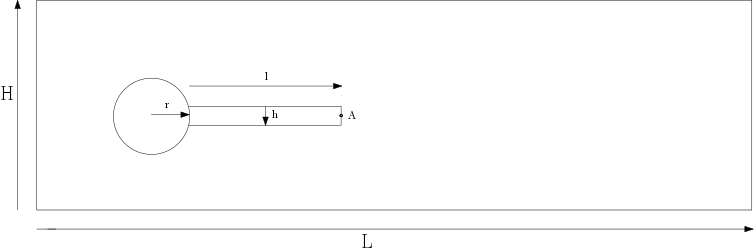
\includegraphics[scale=0.4]{./Verification_Validation/Hron_Turek/Domain_drawing.png}
\end{center}
The computational domain consists of a circle with an elastic bar behind the circle. The circle is positioned at (0.2, 0.2) making it 0.05 of center from bottom to top, this is done to induce oscillations to an otherwise laminar flow. 
This gives a force to the elastic bar. The parameters of the domain are:\\
L = 2.5, H = 0.41, l = 0.35, h = 0.02, A = (0.2,0.6) \\

\subsubsection*{Boundary conditions}
The fluid velocity has a parabolic profile on the inlet that changes over time:\\

\begin{align*}
u(0,y) &= 1.5u_0 \frac{y(H-y)}{(\frac{H}{2})^2}  \\
u(0,y,t) &= u(0,y)\frac{1-cos(\frac{\pi}{2}t)}{2} \text{  for  } t<2.0 \\
u(0,y,t) &= u(0,y) \text{  for  } t \leq 2.0
\end{align*}

We set no slip on the "floor" and "ceiling" so to speak.\\
$$ u(x,y,t) = 0 \text{  on  }  $$
On the fluid solid interface the boundary conditions are set to:
$$  \sigma_f n_f = \sigma_s n_s \hspace{4mm} on  \hspace{2mm}\Gamma^0 (interface)   $$
In our variational form we leave this out and so implying that they are equal.

\subsubsection*{Quantities for comparison}
When the fluid moves around the circle and bar it exerts a force. These are split into drag and lift and calculated as follows:
$$ (F_d, F_L) = \int_S \sigma_f n dS $$ 
where S is the part of the circle and bar in contact with the fluid. \\
We set a point A on the right side of the bar. This point is used to track the deformation in CSM and FSI tests. \\
In each test the numbers with ref are the values taken from the benchmark paper \cite{Hron2006a}
We integrate the mapped fluid stress tensor over the bar and circle and appended to lists: 
\begin{lstlisting}[language=Python]
Dr = -assemble((sigma_f_new(v,p,d,mu_f)*n)[0]*ds(6))
Li = -assemble((sigma_f_new(v,p,d,mu_f)*n)[1]*ds(6))
Dr += -assemble((sigma_f_new(v("-"),p("-"),d("-"),mu_f)*n("-"))[0]*dS(5))
Li += -assemble((sigma_f_new(v("-"),p("-"),d("-"),mu_f)*n("-"))[1]*dS(5))
Drag_list.append(Dr)
Lift_list.append(Li)
\end{lstlisting}
The deformation is calculated on the point A, and also added to lists:
\begin{lstlisting}[language=Python]
dsx = d(coord)[0]
dsy = d(coord)[1]
dis_x.append(dsx)
dis_y.append(dsy)
\end{lstlisting}
\subsection{Results}
\subsubsection*{CFD test}
The first two CFD tests are run with Reynolds number 20 and 100 giving steady drag and lift around the circle. CFD 3 has a Reynolds number 200 which will induce oscillations behind the circle, giving fluctuations in the drag and lift.
The CFD tests were run using the the bar as rigid object, that is the domain calculated is just the fluid domain. It is possible to also calculate with the bar and setting $\rho_s$ and $\mu_s$ to a large value. 

\begin{table}[h!]
\centering
\caption{CFD parameters}
\label{my-label}
\begin{tabular}{|l|l|l|l|}
\hline
Parameters & CFD1 & CFD2 & CFD3 \\ \hline
$\rho_f [10^3 \frac{kg}{m^3}]$ & 1 & 1 & 1 \\ \hline
$\nu_f [10^{-3} \frac{m^2}{s}]$ & 1 & 1 & 1 \\ \hline
$ U [\frac{m}{s}] $ & 0.2 & 1 & 2 \\ \hline
Re = $\frac{Ud}{\nu_f}$ & 20 & 100 & 200 \\ \hline
\end{tabular}
\end{table}

\begin{table}[h!]
\centering
\caption{CFD 1}
\label{my-label}
\begin{tabular}{|l|l|l|l|}
\hline
\textbf{elements} & \textbf{dofs} & \textbf{Drag} & \textbf{Lift} \\ \hline
6616 & 32472 & 14.2439 & 1.0869 \\ \hline
26464 & 124488 & 14.2646 & 1.11085 \\ \hline
105856 & 487152 & 14.2755 & 1.11795 \\ \hline
\textbf{ref} & \textbf{} & \textbf{14.29} & \textbf{1.119} \\ \hline
\end{tabular}
\end{table}

\begin{table}[h!]
\centering
\caption{CFD 2}
\label{my-label}
\begin{tabular}{|l|l|l|l|}
\hline
\textbf{elements} & \textbf{dofs} & \textbf{Drag} & \textbf{Lift} \\ \hline
6616 & 32472 & 135.465 & 6.27158 \\ \hline
26464 & 124488 & 136.566 & 9.82166 \\ \hline
105856 & 487152 & 136.573 & 10.4441 \\ \hline
\textbf{ref} & \textbf{} & \textbf{136.7} & \textbf{10.53} \\ \hline
\end{tabular}
\end{table}

\subsubsection*{CSM test}
The CSM test are calculated using only the bare and adding a gravity term $g$ with the same value but changing the parameters of solid.
As with the CFD test the first to CSM test cause a steady state solution, and CSM 3 is more slender causing the bar to go up and down in time. Our quantity for comparing there will be the deformation of the point $A$. In CSM 3 the energy is conserved by using a Crank-Nicholson scheme as can be seen in the plots fig7 (hvordan citer man et plot?)

\begin{table}[h!]
\centering
\caption{Parameters}
\label{my-label}
\begin{tabular}{|l|l|l|l|}
\hline
Parameters & CSM1 & CSM2 & CSM3 \\ \hline
$\rho_f[10^3 \frac{kg}{m^3}]$ & 1 & 1 & 1 \\ \hline
$\nu_f [10^{-3} \frac{m^2}{s}]$ & 1 & 1 & 1 \\ \hline
$u_0$ & 0 & 0 & 0 \\ \hline
$\rho_s[10^3 \frac{kg}{m^3}]$ & 1 & 1 & 1 \\ \hline
$\nu_s$ & 0.4 & 0.4 & 0.4 \\ \hline
$\mu_s[10^6 \frac{m^2}{s}]$ & 0.5 & 2.0 & 0.5 \\ \hline
$g $ & 2 & 2 & 2 \\ \hline
\end{tabular}
\end{table}

\begin{table}[h!]
\centering
\caption{CSM 1}
\label{my-label}
\begin{tabular}{|l|l|l|l|}
\hline
elements & dofs & ux $[10^{?3}]$ & uy $[10^{?3}]$ \\ \hline
725 & 1756 & -5.80951654915 & -59.4781430115 \\ \hline
2900 & 6408 & -6.77960453995 & -64.2130757639 \\ \hline
11600 & 24412 & -7.08597041285 & -65.635825349 \\ \hline
46400 & 95220 & -7.11626976966 & -65.7456687273 \\ \hline
ref & ref & -7.187 & -66.10 \\ \hline
\end{tabular}
\end{table}

% Please add the following required packages to your document preamble:
% \usepackage{booktabs}
\begin{table}[h!]
\centering
\caption{CSM 2}
\label{my-label}
\begin{tabular}{@{}|l|l|l|l|@{}}
\hline
Elements & Dofs & ux $[10^{-3}] $& ux $[10^{-3}] $\\ \hline
725 &  1756 & -0.375962146908 & -15.1950342598 \\ \hline
2900 & 6408 & -0.441308781709 & -16.4643196042\\ \hline
11600 & 24412 & -0.462087305294 & -16.8478689583 \\ \hline
46400 & 95220 & -0.464128022327 & -16.8782135872\\ \hline
ref & ref & -0.4690 & -16.97 \\ \hline
\end{tabular}
\end{table}

\begin{table}[h!]
\centering
\caption{CSM 3}
\label{my-label}
\begin{tabular}{|l|l|l|l|}
\hline
elements & dofs & ux $[10^3]$ & uy $[10^3]$ \\ \hline
725 & 1756 & $-11.743 \pm 11.744$ & $-57.952 \pm 58.940$ \\ \hline
2900 & 6408 & $-13.558 \pm 13.559$ & $ -61.968 \pm  63.440 $ \\ \hline
11600 & 24412 & $ -14.128 \pm 14.127$ & $-63.216 \pm 64.744 $ \\ \hline
46400 & 95220 & $ -14.182 \pm 14.181 $ & $ -63.305 \pm 64.843 $ \\ \hline
ref &  & $-14.305 \pm 14.305 $ & $-63.607 \pm 65.160 $ \\ \hline
\end{tabular}
\end{table}

\begin{figure}[h!] 
  \begin{subfigure}[b]{0.5\linewidth}
    \centering
    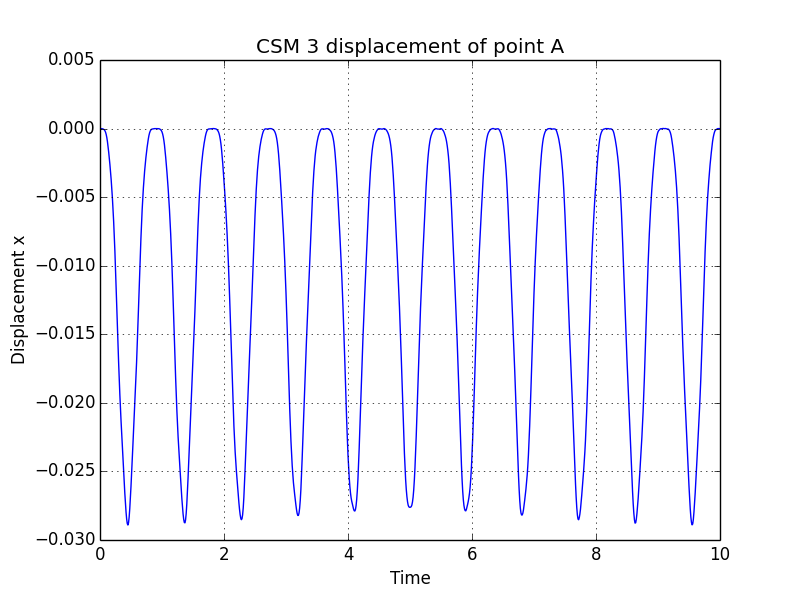
\includegraphics[width=0.75\linewidth]{./Verification_Validation//Hron_Turek/dis_x.png} 
    \caption{Displacement in x-direction} 
    \label{fig7:a} 
    \vspace{4ex}
  \end{subfigure}%% 
  \begin{subfigure}[b]{0.5\linewidth}
    \centering
    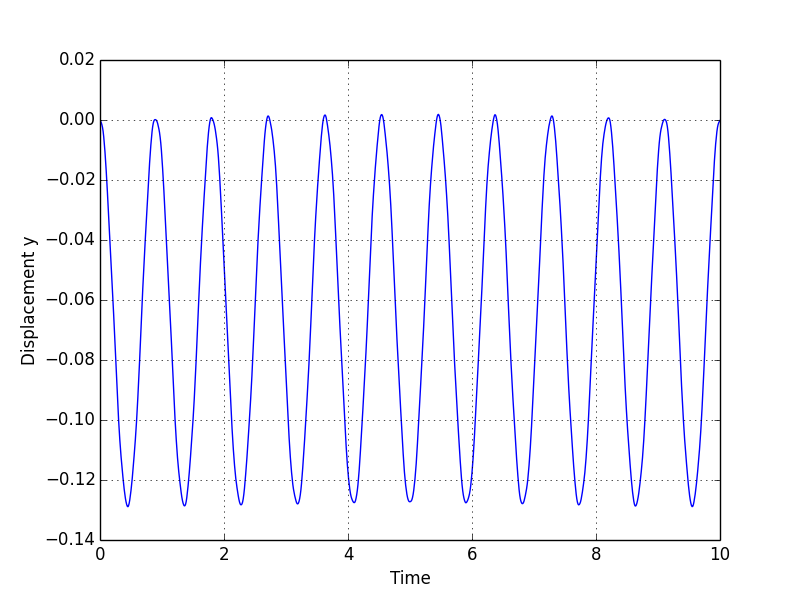
\includegraphics[width=0.75\linewidth]{./Verification_Validation//Hron_Turek/dis_y.png} 
    \caption{Displacement in x-direction} 
    \label{fig7:b} 
    \vspace{4ex}
  \end{subfigure} 
  \begin{subfigure}[b]{0.5\linewidth}
    \centering
    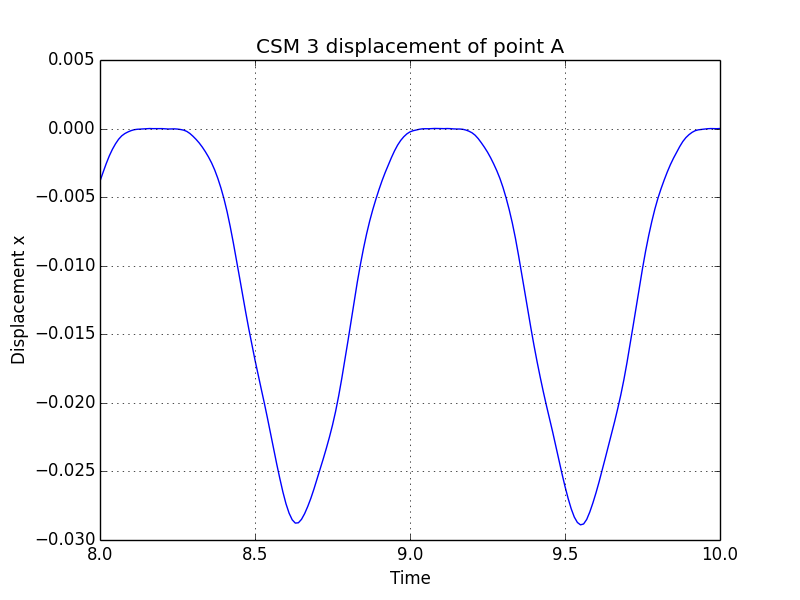
\includegraphics[width=0.75\linewidth]{./Verification_Validation//Hron_Turek/dis_x_short.png} 
    \caption{Displacement in x-direction} 
    \label{fig7:c} 
  \end{subfigure}%%
  \begin{subfigure}[b]{0.5\linewidth}
    \centering
    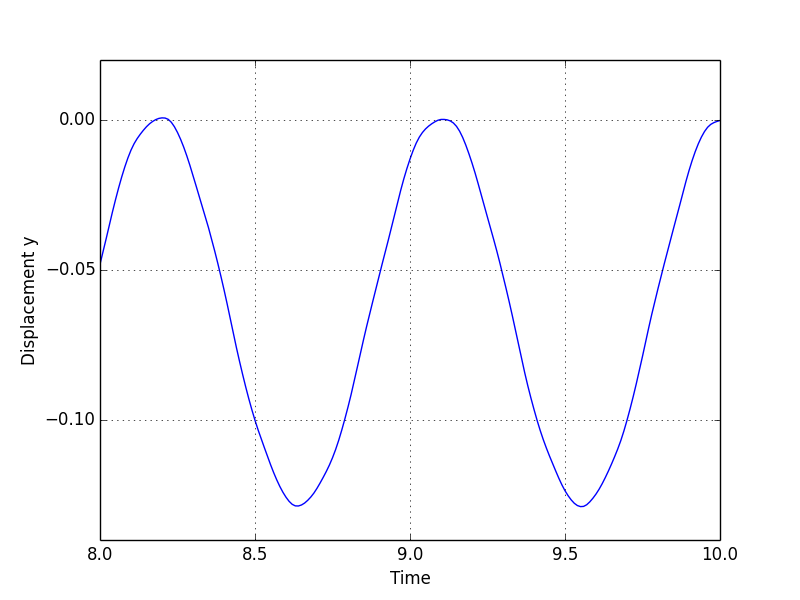
\includegraphics[width=0.75\linewidth]{./Verification_Validation/Hron_Turek/dis_y_short.png} 
    \caption{Displacement in x-direction} 
    \label{fig7:d} 
  \end{subfigure} 
  \caption{Displacement of point A}
  \label{fig7} 
\end{figure}


\subsection*{FSI test}
\begin{table}[ht]
\centering
\caption{FSI Parameters}
\label{my-label}
\begin{tabular}{|l|l|l|l|}
\hline
Parameters & FSI1 & FSI2 & FSI3 \\ \hline
$\rho_f[10^3 \frac{kg}{m^3}]$ & 1 & 1 & 1 \\ \hline
$\nu_f [10^{-3} \frac{m^2}{s}]$ & 1 & 1 & 1 \\ \hline
$u_0$ & 0.2 & 1 & 2 \\ \hline
Re = $\frac{U d}{\nu_f}$ & 20 & 100 & 200 \\ \hline
$\rho_s[10^3 \frac{kg}{m^3}]$ & 1 & 10 & 1 \\ \hline
$\nu_s$ & 0.4 & 0.4 & 0.4 \\ \hline
$\mu_s[10^6 \frac{m^2}{s}]$ & 0.5 & 0.5 & 2 \\ \hline
\end{tabular}
\end{table}
Results: 
\begin{table}[h]
\centering
\caption{FSI 1}
\label{my-label}
\begin{tabular}{|l|l|l|l|l|l|l|}
\hline
Cells & Dofs & ux of A $[x10^{-3}]$ & uy of A $[x10^{-3}]$ & Drag & Lift & Spaces \\ \hline
2698 & 7095 & 0.0234594 & 0.797218  & 14.4963 & 0.915801 & P1-P1-P1 stab= 0.01 \\ \hline
2698 & 23563 &0.0227418 &0.799314  &  14.1735 &0.761849 & P2-P2-P1 \\ \hline
10792 & 92992  &0.0227592 & 0.80795 & 14.1853 &  0.775063 &  P2-P2-P1 \\ \hline
43168 & 369448 & 00.227566 & 0.813184 & 14.2269 & 0.771071 & P2-P2-P1 \\ \hline
\textbf{ref} & \textbf{ref} & \textbf{0.0227} & \textbf{0.8209} & \textbf{14.295} & \textbf{0.7638} & \textbf{ref} \\ \hline
\end{tabular}
\end{table}



\newpage
OLD SHITZ FSI:
\begin{table}[h]
\centering
\caption{FSI 1}
\label{my-label}
\begin{tabular}{|l|l|l|l|l|l|l|}
\hline
Cells & Dofs & ux of A $[x10^{-3}]$ & uy of A $[x10^{-3}]$ & Drag & Lift & Spaces \\ \hline
2698 & 7095 & 0.0234594 & 0.797218  & 14.4963 & 0.915801 & P1-P1-P1 stab= 0.01 \\ \hline
2698 & 23563 & 0.02271 & 0.80288 & 14.1736 & 0.787891 & P2-P2-P1 \\ \hline
2698 & 23563 & 0.00581116 & 0.000000738678  & 12.07 & 0.02345 & P2-P2-P1 without weighting \\ \hline
10792 & 92992 & 0.0227341 & 0.808792 & 14.1855 & 0.801044 & P2-P2-P1 \\ \hline
43168 & 369448 & 0.227352 & 0.812595 & 14.227 & 0.797242 & P2-P2-P1 \\ \hline
\textbf{ref} & \textbf{ref} & \textbf{0.0227} & \textbf{0.8209} & \textbf{14.295} & \textbf{0.7638} & \textbf{ref} \\ \hline
\end{tabular}
\end{table}
\subsection{Comparing different lifting operators}\label{sec:mesh_motion}
This section is devoted to comparing different lifting operators from \ref{sec:meshmotion}. The comparisions will be run using a version of the CSM test discussed earlier, with the same computing domain as the Hron Turek benchmark. The tests will compare the different techniques by looking at the how the deformation is lifted into the fluid domain. This is done by investigating a plot of the mesh after deformation to see how much cells distort and where the cells distort. This is visualized using Paraview.\newline
In these test cases we have the fluid initially at rest and with no inflow on the fluid. A gravitational force is applied to the structure much like the previous CSM test. The only difference is that we now use the full domain from the \ref{sec:HronTurek} . The tests are run as time-dependent with a the backward Euler scheme, leading to a steady state solution. In the first test case the parameters from CSM1 are used, and in the CSM4 the gravitational force has just been increased from 2 to 4. \newline

A plot has been added at the end of the FSI2 case run with different techniques to investigate the impact these have on the overall FSI problem.

\subsection*{Boundary conditions}
The upper, lower and left boundary is set as no slip, that is no velocity in the fluid. On the left boundary there is a do nothing, and zero pressure. 
\subsection*{Quantities for comparison}
The different techniques will be plotted with the minimal value of the Jacobian. The Jacobian determinant of the deformation rate, and \textbf{if the Jacobian is zero anywhere in the domain it means that the cells overlap and can cause singularity in the matrices during assembly.} \newline
We will also look at the a plot of the deformation in the domain, to visualize how the different mesh motion techniques work. It is possible to see that if get thin triangles in the computational domain then the lifting operator is not good enough.
\subsubsection*{CSM1}
\begin{figure}[H]
\label{fig:fluid_structure}
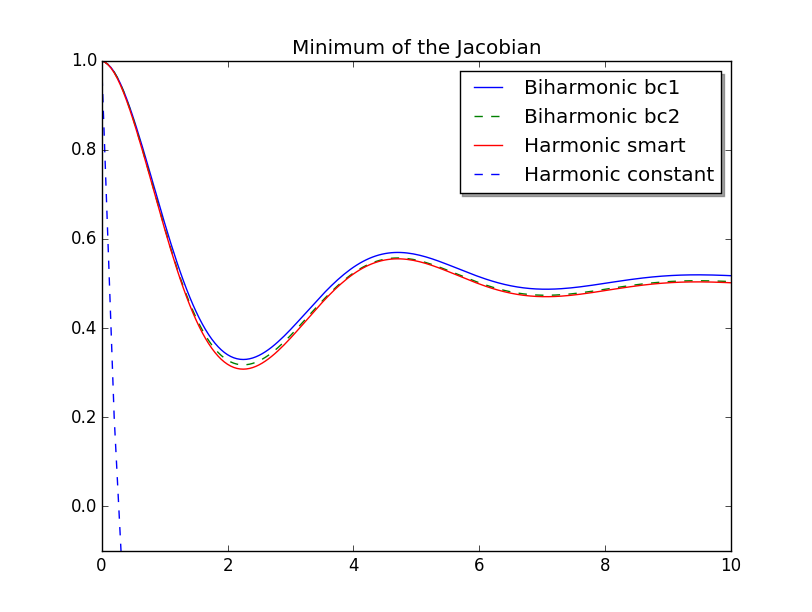
\includegraphics[scale=0.60, trim={0mm 0mm 0mm 0mm},clip]{./Verification_Validation/Mesh_motion_results/CSM1.png}
\caption{min J of the CSM1 test}
\end{figure}

\begin{figure}[H]  \label{fig:CSM1_pictures} 
  \caption{Results of testing different lifting operator using the CSM1 testcase computing full FSI}
  \begin{minipage}[b]{0.6\linewidth}
    \centering
    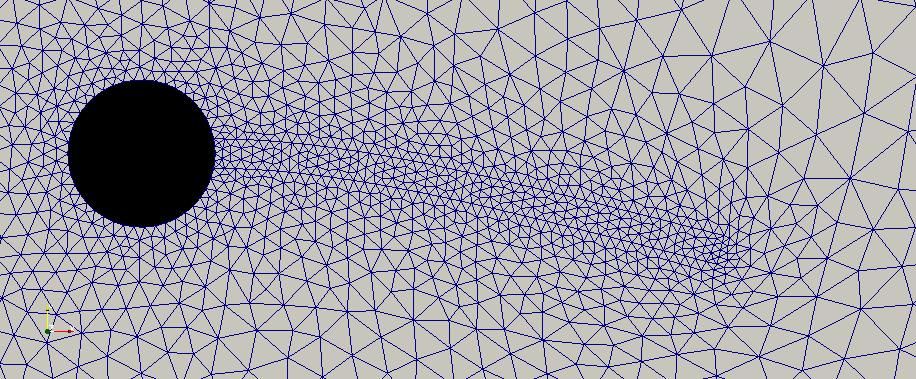
\includegraphics[scale=0.25]{./Verification_Validation/Mesh_motion_results/CSM1_laplace.png} 
    \caption{Harmonic smart} 
    \vspace{4ex}
  \end{minipage}%%
  \begin{minipage}[b]{0.6\linewidth}
    \centering
    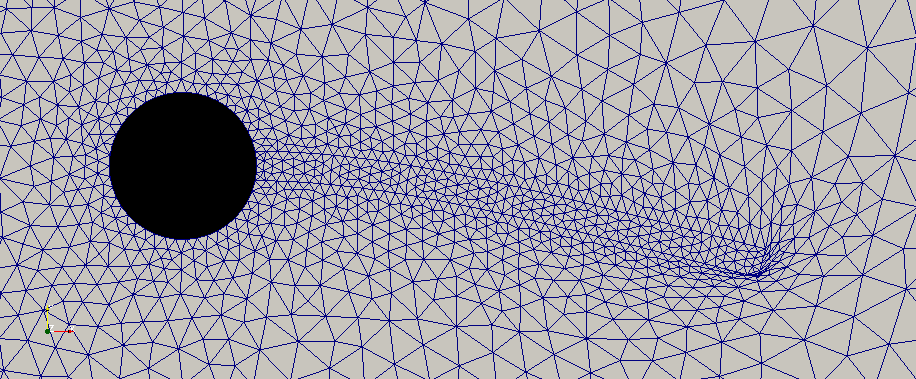
\includegraphics[scale=0.25]{./Verification_Validation/Mesh_motion_results/CSM1_constant.png} 
    \caption{Harmonic constant} 
    \vspace{4ex}
  \end{minipage} 
  \begin{minipage}[b]{0.6\linewidth}
    \centering
    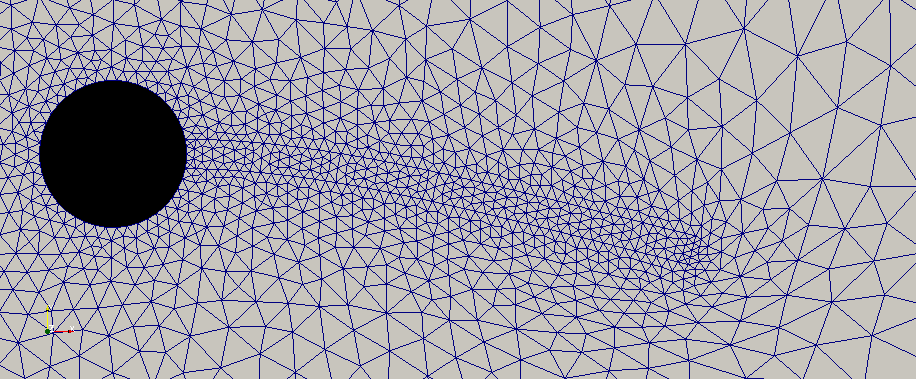
\includegraphics[scale=0.25]{./Verification_Validation/Mesh_motion_results/CSM1_bibc1.png} 
    \caption{Biharmonic bc1} 
    \vspace{4ex}
  \end{minipage}%% 
  \begin{minipage}[b]{0.6\linewidth}
    \centering
    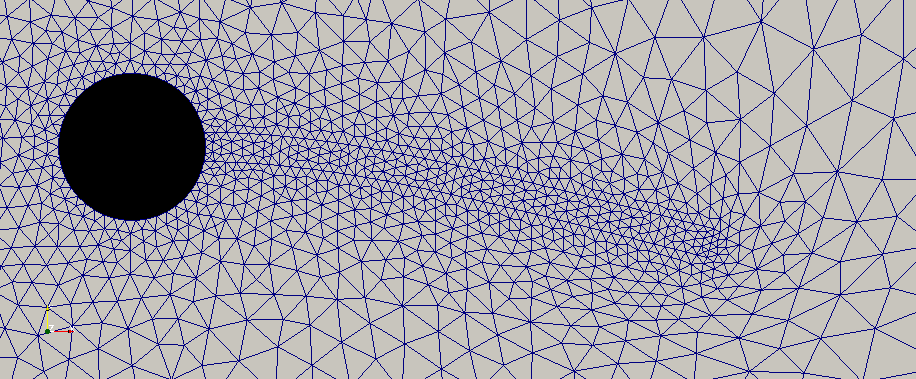
\includegraphics[scale=0.25]{./Verification_Validation/Mesh_motion_results/CSM1_bibc2.png} 
    \caption{Biharmonic bc2} 
    \vspace{4ex}
  \end{minipage} 
\end{figure}



\begin{table}[H]
\centering
\caption{Displacements results of different lifting operators of CSM1 test}
\label{my-label}
\begin{tabular}{|l|l|l|}
\hline
Technique & $d_y(A) [\times 10^{-3}]$ & $d_x(A) [\times 10^{-3}]$ \\ \hline
Harmonic & 65.406 & 7.036 \\ \hline
Constant & 43.033 & 2.999 \\ \hline
Bibc1 & 65.404 & 7.036 \\ \hline
Bibc2 & 65.405 & 7.036 \\ \hline
\end{tabular}
\end{table}


Looking at figure \ref{fig:fluid_structure} which shows the minimum of the Jacobian of the entire domain. The Harmonic with a constant $\alpha_u$ parameter. Gives overlapping cells quickly and computations stop.
While the harmonic named smart meaning an $\alpha_u$ that is greater closer to the interface, and both the biharmonic techniques gives good and similar results. All three uphold, as we can see in \ref{fig:CSM1_pictures}, the integrity of the cells.


\subsubsection{FSI2 with Lifting operator}

\begin{figure}[H]  \label{fig:FSI2_motion} 
  \begin{minipage}[b]{0.5\linewidth}
    \centering
    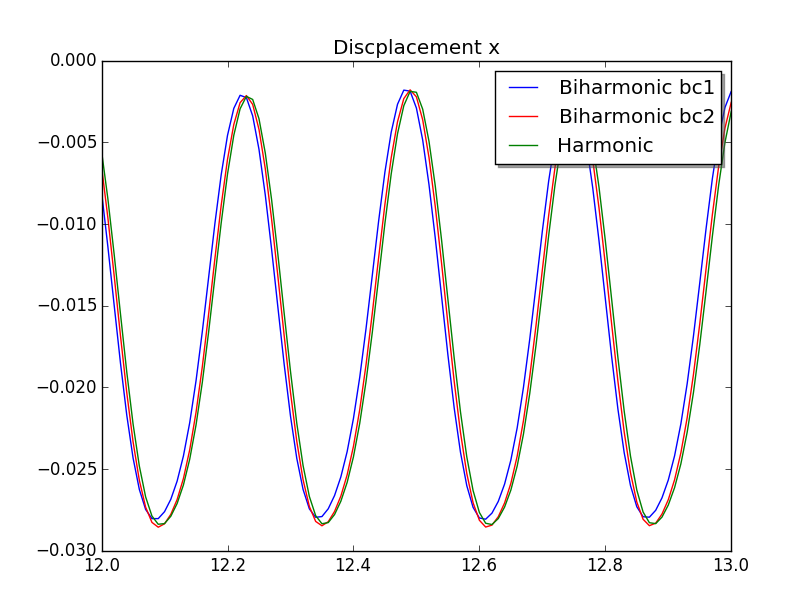
\includegraphics[scale=0.35]{./Verification_Validation/Mesh_motion_results/FSI2_dt001_dis_x.png} 
    \vspace{4ex}
  \end{minipage}%%
  \begin{minipage}[b]{0.5\linewidth}
    \centering
    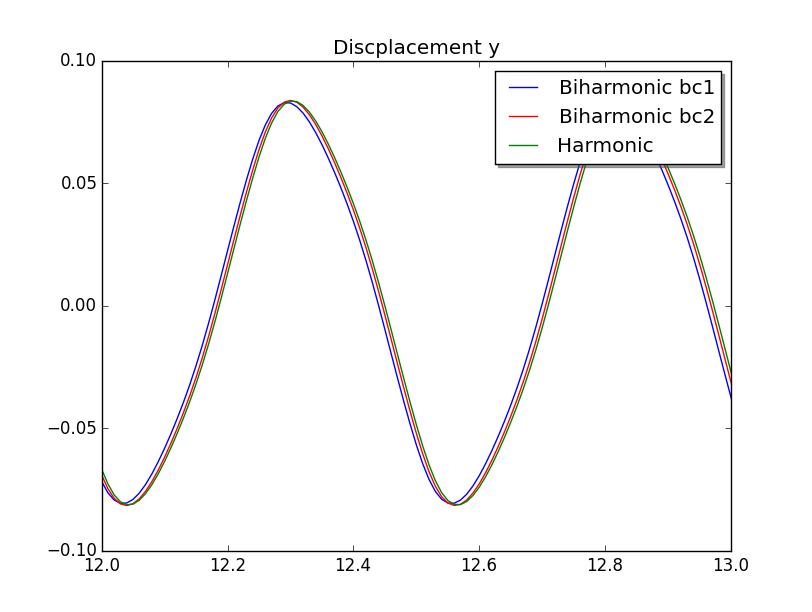
\includegraphics[scale=0.35]{./Verification_Validation/Mesh_motion_results/FSI2_dt001_dis_y.png} 
    \vspace{4ex}
  \end{minipage} 
  \begin{minipage}[b]{0.5\linewidth}
    \centering
    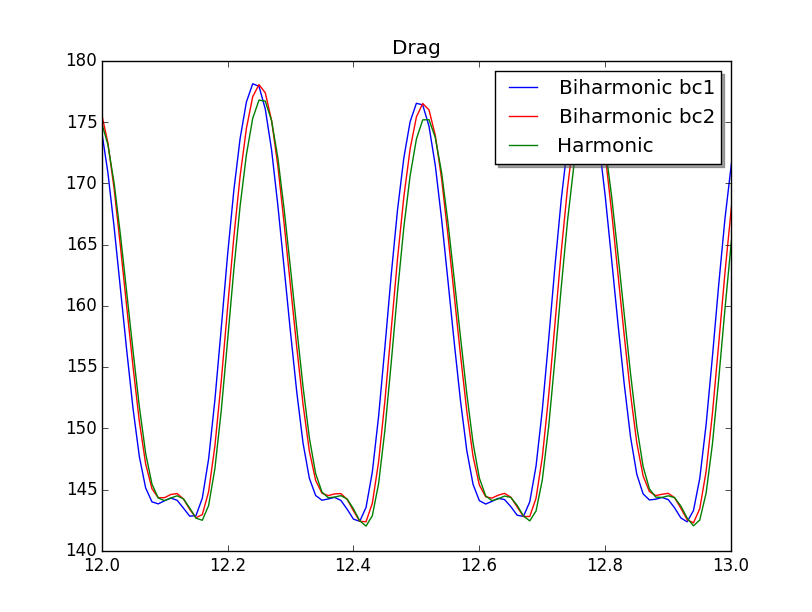
\includegraphics[scale=0.35]{./Verification_Validation/Mesh_motion_results/FSI2_dt001_drag.png} 
    \vspace{4ex}
  \end{minipage}%% 
  \begin{minipage}[b]{0.5\linewidth}
    \centering
    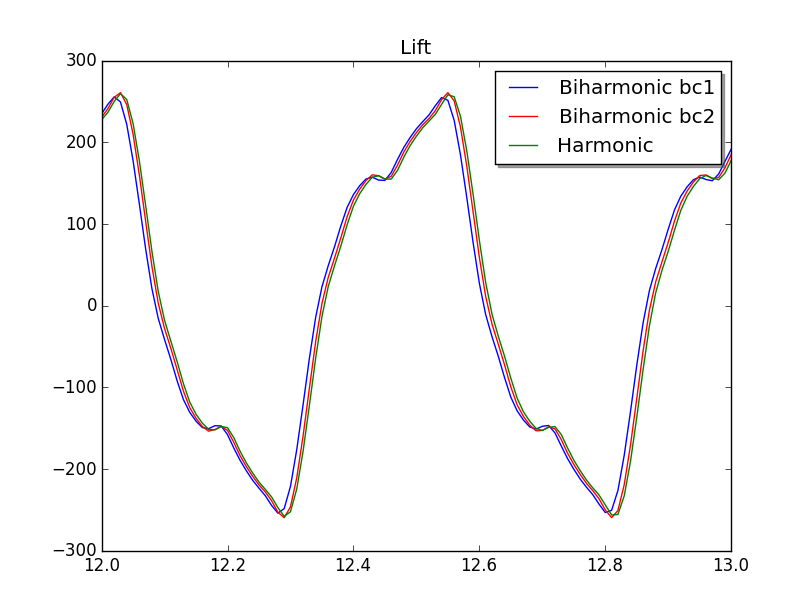
\includegraphics[scale=0.35]{./Verification_Validation/Mesh_motion_results/FSI2_dt001_lift.png} 
    \vspace{4ex}
  \end{minipage} 
\caption {FSI2 with different lifting operators: Harmonic, Biharmonic bc1 and bc2. $\Delta t = 0.01$}
\end{figure}

Figure \ref{fig:FSI2_motion} shows the harmonic and the two biharmonic mesh motion techniques for the FSI2 case. All three are similar and only a slight change in the period can be noticed. This indicates that with a clever $\alpha_u$ the harmonic technique can be chosen. This is an advantage since the harmonic techniques is the least computationally costly.









\section{Investigating Numerical Stability for Fluid-Structure Interaction Problems}
The following section will give a brief insight in to the effects of choosing different $\theta$ values in the $\theta-$scheme for different time steps. 
The benchmark tests FSI2 and FSI3, as discussed in the previous section, has been investigated since they are known to be numerical unstable for certain values of $\theta$ and $\Delta t$. Only the effects of Drag are reported as the three other quantities shows similar behavior. 
The impact of different $\theta$ values on energy stability in the solid mechanical benchmark CSM3 is also investigated.
\newpage

Figure \ref{fig:FSI2drag_plots} shows the temporal evolution of drag in a simulation with $\Delta t = 0.01$. In the left panel the results are from simulations with $\theta = 0.5 + \Delta t$, and in the right panel $\theta = 0.5$. Based on the results we can observe that a standard Crank-Nicholson scheme becomes unstable when reaching $\sim$13 s. While the shifted Crank-Nicholson,  $\theta = 0.5 + \Delta t$, is stable throughout the simulation.

\begin{figure}[H] 
  \begin{minipage}[b]{0.6\linewidth}
    \centering
    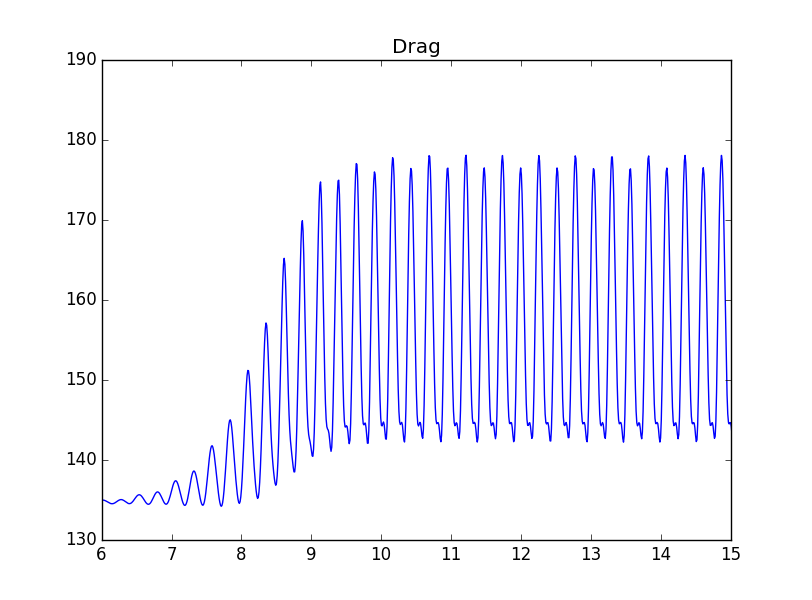
\includegraphics[scale=0.40]{./Temporal_stability/FSI2_001_051_big.png} 
    \caption{Drag vs time with $\theta = 0.50 + \Delta t $} 
    \vspace{4ex}
  \end{minipage}%%
  \begin{minipage}[b]{0.6\linewidth}
    \centering
    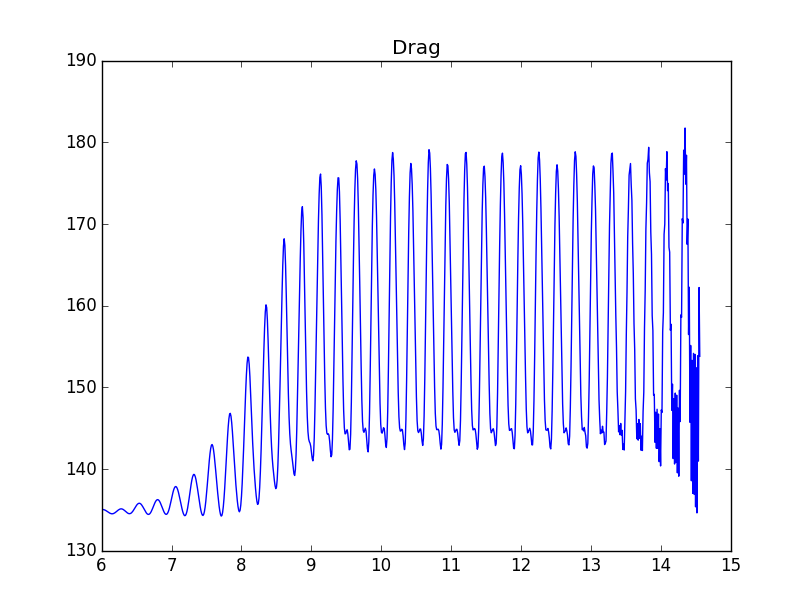
\includegraphics[scale=0.40]{./Temporal_stability/FSI2_001_050_big.png} 
    \caption{Drag vs time with $\theta = 0.50 $} 
    \vspace{4ex}
  \end{minipage} 
  \begin{minipage}[b]{0.6\linewidth}
    \centering
    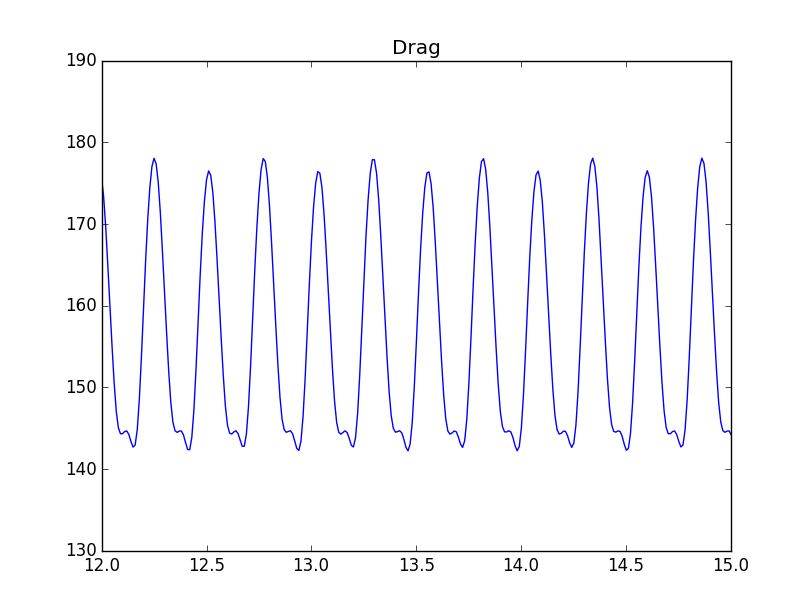
\includegraphics[scale=0.40]{./Temporal_stability/FSI2_001_051_small.png} 
    \caption{Drag vs time with $\theta = 0.50 +\Delta t $} 
    \vspace{4ex}
  \end{minipage}%% 
  \begin{minipage}[b]{0.6\linewidth}
    \centering
    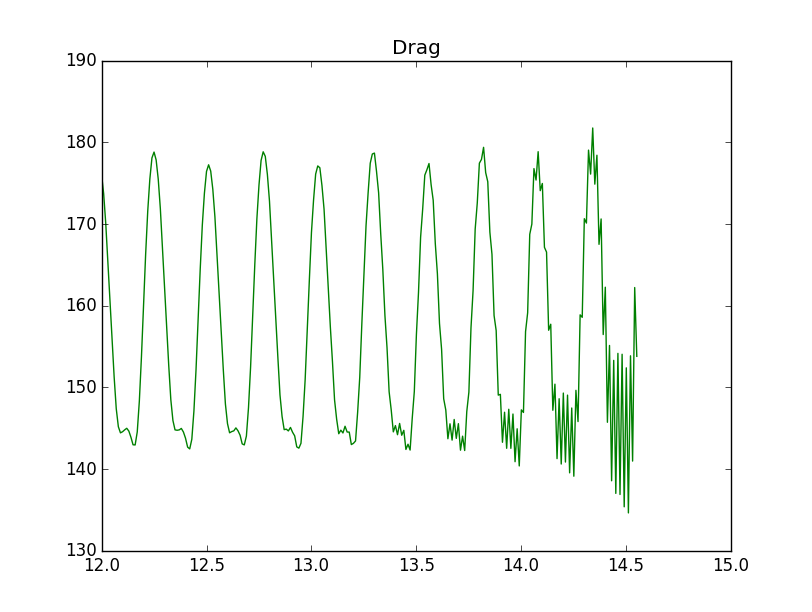
\includegraphics[scale=0.40]{./Temporal_stability/FSI2_001_050_small.png} 
    \caption{Drag vs time with $\theta = 0.50 $} 
    \vspace{4ex}
  \end{minipage} 
\caption {Drag for FSI2 with $\Delta t = 0.01$ with different values for $\theta$}
\label{fig:FSI2drag_plots} 
\end{figure}

Figures \ref{fig: FSI3_long_short} show drag for FSI3 simulation with $\Delta t = 0.001$ and $\theta = 0.5$, showing long term stability for the normal Crank-Nicholson scheme.

\begin{figure}[H]
\begin{tabular}{ll}
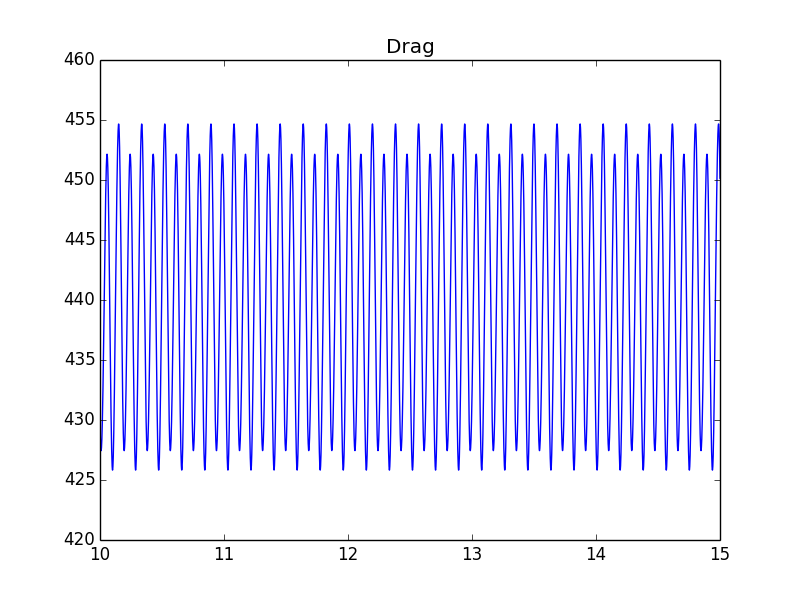
\includegraphics[scale=0.4]{./Temporal_stability/FSI3_0001_050_big.png}
&
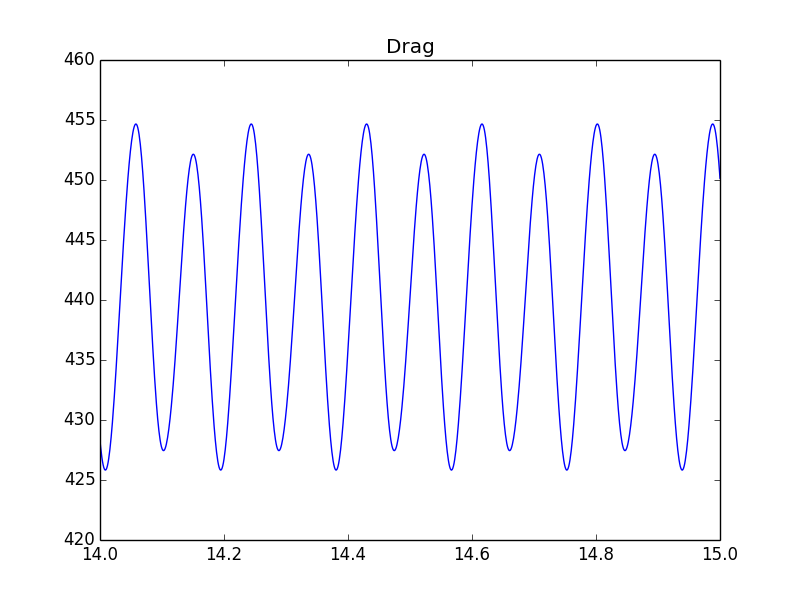
\includegraphics[scale=0.4]{./Temporal_stability/FSI3_0001_050_small.png}
\end{tabular}
\caption{FSI3 drag vs time plot for 10-15 seconds and 14-15 seconds, with $\Delta t = 0.001$ and $\theta =0.5$ showing long term numerical stability}
\label{fig: FSI3_long_short}
\end{figure}

For the CSM3 case only the solid bar is computed, and with an applied force g and no friction, the bar should move down and back up infinitely, for a correct solution.

Figure \ref{fig:CSM3_dis_plots} shows plots of the displacements in x and y directions for $\theta = 0.5$ and $1$. With the implicit scheme ($\theta=1$) the bar moves to a steady state solution. This means energy has not been preserved and the energy dissipates. While in the Crank-Nicholson scheme ($\theta = 0.5$), the bar moves down and back up. This indicates that the Crank-Nicholson scheme is energy preserving.

\begin{figure}[H] 
  \begin{minipage}[b]{0.6\linewidth}
    \centering
    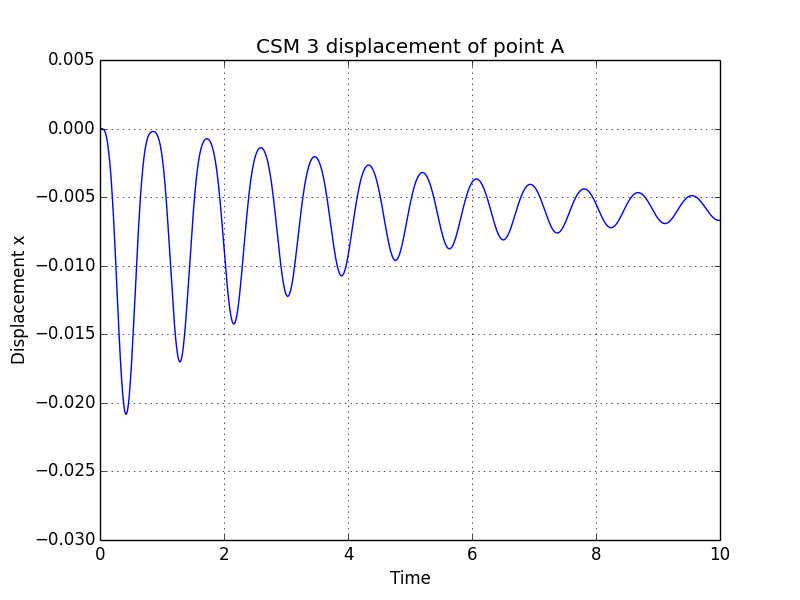
\includegraphics[scale=0.40]{./Temporal_stability/CSM3_implicit.png} 
    \caption{$\theta = 1 $} 
    \vspace{4ex}
  \end{minipage}%%
  \begin{minipage}[b]{0.6\linewidth}
    \centering
    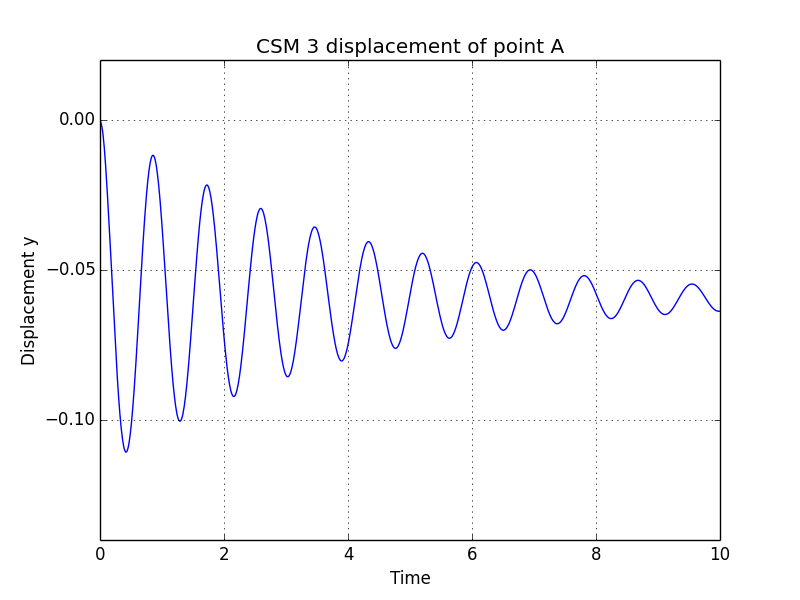
\includegraphics[scale=0.40]{./Temporal_stability/CSM3_implicit_y.png} 
    \caption{$\theta = 1 $} 
    \vspace{4ex}
  \end{minipage} 
  \begin{minipage}[b]{0.6\linewidth}
    \centering
    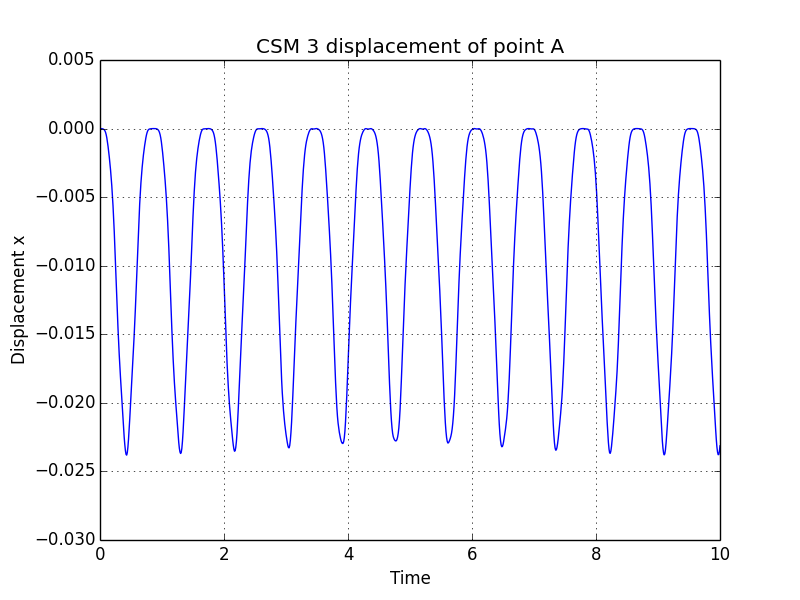
\includegraphics[scale=0.40]{./Temporal_stability/CSM3_Crank.png} 
    \caption{$\theta = 0.5 $} 
    \vspace{4ex}
  \end{minipage}%% 
  \begin{minipage}[b]{0.6\linewidth}
    \centering
    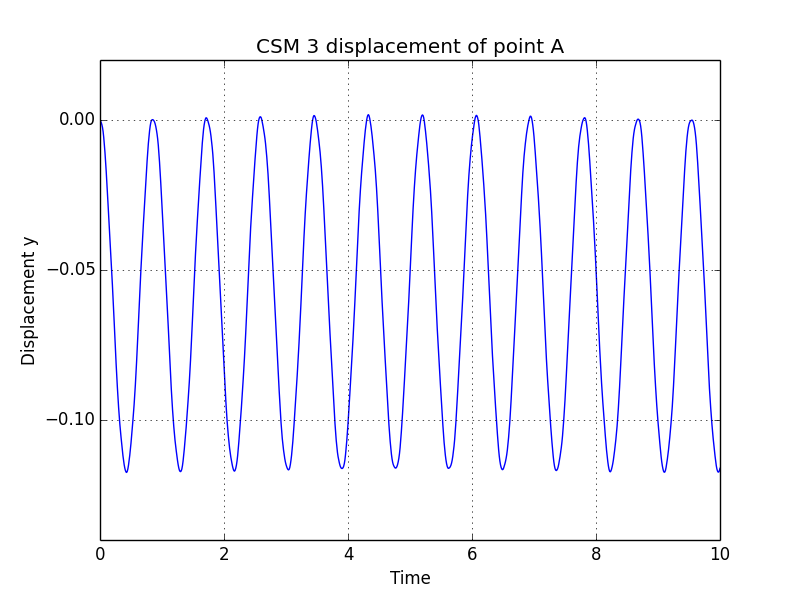
\includegraphics[scale=0.40]{./Temporal_stability/CSM3_Crank_y.png} 
    \caption{$\theta = 0.5 $} 
    \vspace{4ex}
  \end{minipage} 
 \label{fig:CSM3_dis_plots} 
 \caption {CSM3 displacements with $\Delta t = 0.01$ with different values for $\theta$}
\end{figure}


\subsubsection*{Discussion on numerical stability}
The shifted version of the Crank-Nicholson scheme is stable when computing for time step values as low as $\Delta t = 0.01$. However with $\Delta t = 0.001$ the normal Crank-Nicholson scheme ($\theta =0.5$) can be used and is long term stable in the period investigated here. It might be that after 100 s, that the flow would become unstable. However, a rigorous investigation of long-term stability is out of the scope of this thesis. 
It has also been reported by Wick 2011 \cite{Wick2011} that the Crank-Nicholson, $\theta = 0.5$, scheme is stable throughout the computing time by setting $\Delta t = 0.001$.

In the FSI2 case the results for the finest mesh showed, in previous chapter, similar results for $\Delta t = 0.01$ and $\Delta t = 0.001$, meaning that the shifted version of the Crank-Nicholson scheme can be applied, in certain cases, with $\Delta t = 0.01$ greatly reducing computational runtime.

The CSM3 test shows that choosing $\theta = 0.5$ is crucial for preserving energy when computing solid problems. The same property will also be present in a FSI simulation, therefore it is crucial that an energy preserving scheme is applied, otherwise one does not have any control over the artificial numerical dissipation.















